\documentclass{beamer}

\usetheme{simple}

\usepackage{scalerel,xparse}
\usepackage{lmodern}
\usepackage[scale=2]{ccicons}
\usepackage{ulem}
\usepackage{tikz}
\usetikzlibrary{positioning,calc,automata}
\usepackage{algorithm}
\usepackage{algorithmic}
\usepackage{caption}
\usepackage{listings}
\usepackage{xcolor, enumitem}
\usepackage{hyperref}

% Watermark background (simple theme)
\setlength{\parindent}{0cm}
\setwatermark{
\includegraphics[height=8cm]{img/chungus.png}}

\NewDocumentCommand\emojisushi{}{
    
\includegraphics{img/1f363.png}
}
\NewDocumentCommand\emojimoyai{}{
    
\includegraphics{img/1f5ff.png}
}   
\NewDocumentCommand\emojicarrot{}{
    
\includegraphics[width=0.3cm]{img/1f955.png}
}   
\NewDocumentCommand\emojiflushed{}{
    
\includegraphics[width=0.3cm]{img/1f633.png}
}   
\NewDocumentCommand\emojisunglasses{}{
    
\includegraphics[width=0.3cm]{img/1f60e.png}
}   
\NewDocumentCommand\emojijuice{}{
    
\includegraphics[width=0.3cm]{img/1f9c3.png}
}   


\title{CSC363 Tutorial 10}
\subtitle{This will take like 40 mins, i'm guessing?}
\date{\today}
\author{Paul ``sushi{\textunderscore}enjoyer'' Zhang}
\institute{University of Chungus in Japanese dub}

\begin{document}

\maketitle

\begin{frame}{Learning objectives this tutorial}
By the end of this tutorial, you should...
\begin{itemize}
\item Have an intuitive understanding of what co-NP is.
\item Be able to define what NP-hard is, and appreciate proofs of NP-hardness, because ironically proving NP-hardness is easier than proving NP-completeness.
\item Be a master of the famous ``educational'' game \textit{Kahoot}, which is much more enjoyable than amogus. 
\end{itemize}

Big Chungus certified readings: what readings? lol. the lecture hasn't even happened yet.
\end{frame}

\begin{frame}{
\includegraphics{img/a.png}}
\begin{figure}[h]
\centering

\includegraphics[width=10cm]{img/helpme.png}

oh no... not again ;-;
\end{figure}

so uh, i hope youse like kahoot! i dunno what else i could cover... :(\footnote{last year when i was taking CSC363 and everything moved online, tutorials were just straight up cancelled! D:}
\end{frame}

\begin{frame}{NP-hard \emojiflushed}
mmm... I briefly mentioned this definition verbally in the last tutorial, but I don't know if any of you remember D:

\vspace{2mm}

\textbf{Recall (maybe):} A language $A$ is \textbf{NP-complete} if \begin{enumerate}[label=(\alph*)]
\item $A \in \text{NP}$;
\item For every $B \in \text{NP}$, $B \leq_p A$.
\end{enumerate}

\vspace{2mm}

Now, sometimes we \sout{get lazy in proving some problem is NP-complete and forget to prove (a)} are unable to prove (a) easily. You'll see some examples later. Despite that, we might still be able to prove (b)! 

\vspace{2mm}

\textbf{Definition:} A language $A$ is \textbf{NP-hard} if for every $B \in \text{NP}$, $B \leq_p A$.

\end{frame}

\begin{frame}{NP-hard \emojiflushed}
mmm... I briefly mentioned this definition verbally in the last tutorial, but I don't know if any of you remember D:

\vspace{2mm}

\textbf{Recall (maybe):} A language $A$ is \textbf{NP-complete} if \begin{enumerate}[label=(\alph*)]
\item $A \in \text{NP}$;
\item For every $B \in \text{NP}$, $B \leq_p A$.
\end{enumerate}

\vspace{2mm}

Now, sometimes we \sout{get lazy in proving some problem is NP-complete and forget to prove (a)} are unable to prove (a) easily. You'll see some examples later. Despite that, we might still be able to prove (b)! 

\vspace{2mm}

\textbf{Definition:} A language $A$ is \textbf{NP-hard} if for every $B \in \text{NP}$, $B \leq_p A$.

\end{frame}

\begin{frame}{NP-hard \emojiflushed}

Now, sometimes we \sout{get lazy in proving some problem is NP-complete and forget to prove (a)} are unable to prove (a) easily. You'll see some examples later. Despite that, we might still be able to prove (b)! 

\vspace{2mm}

\textbf{Definition:} A language $A$ is \textbf{NP-hard} if for every $B \in \text{NP}$, $B \leq_p A$.

\vspace{2mm}

\textbf{Task:} speedrun proving $\text{NP-complete} \subseteq \text{NP-hard}$ fullmarks\%. 

\begin{figure}[h]
\centering
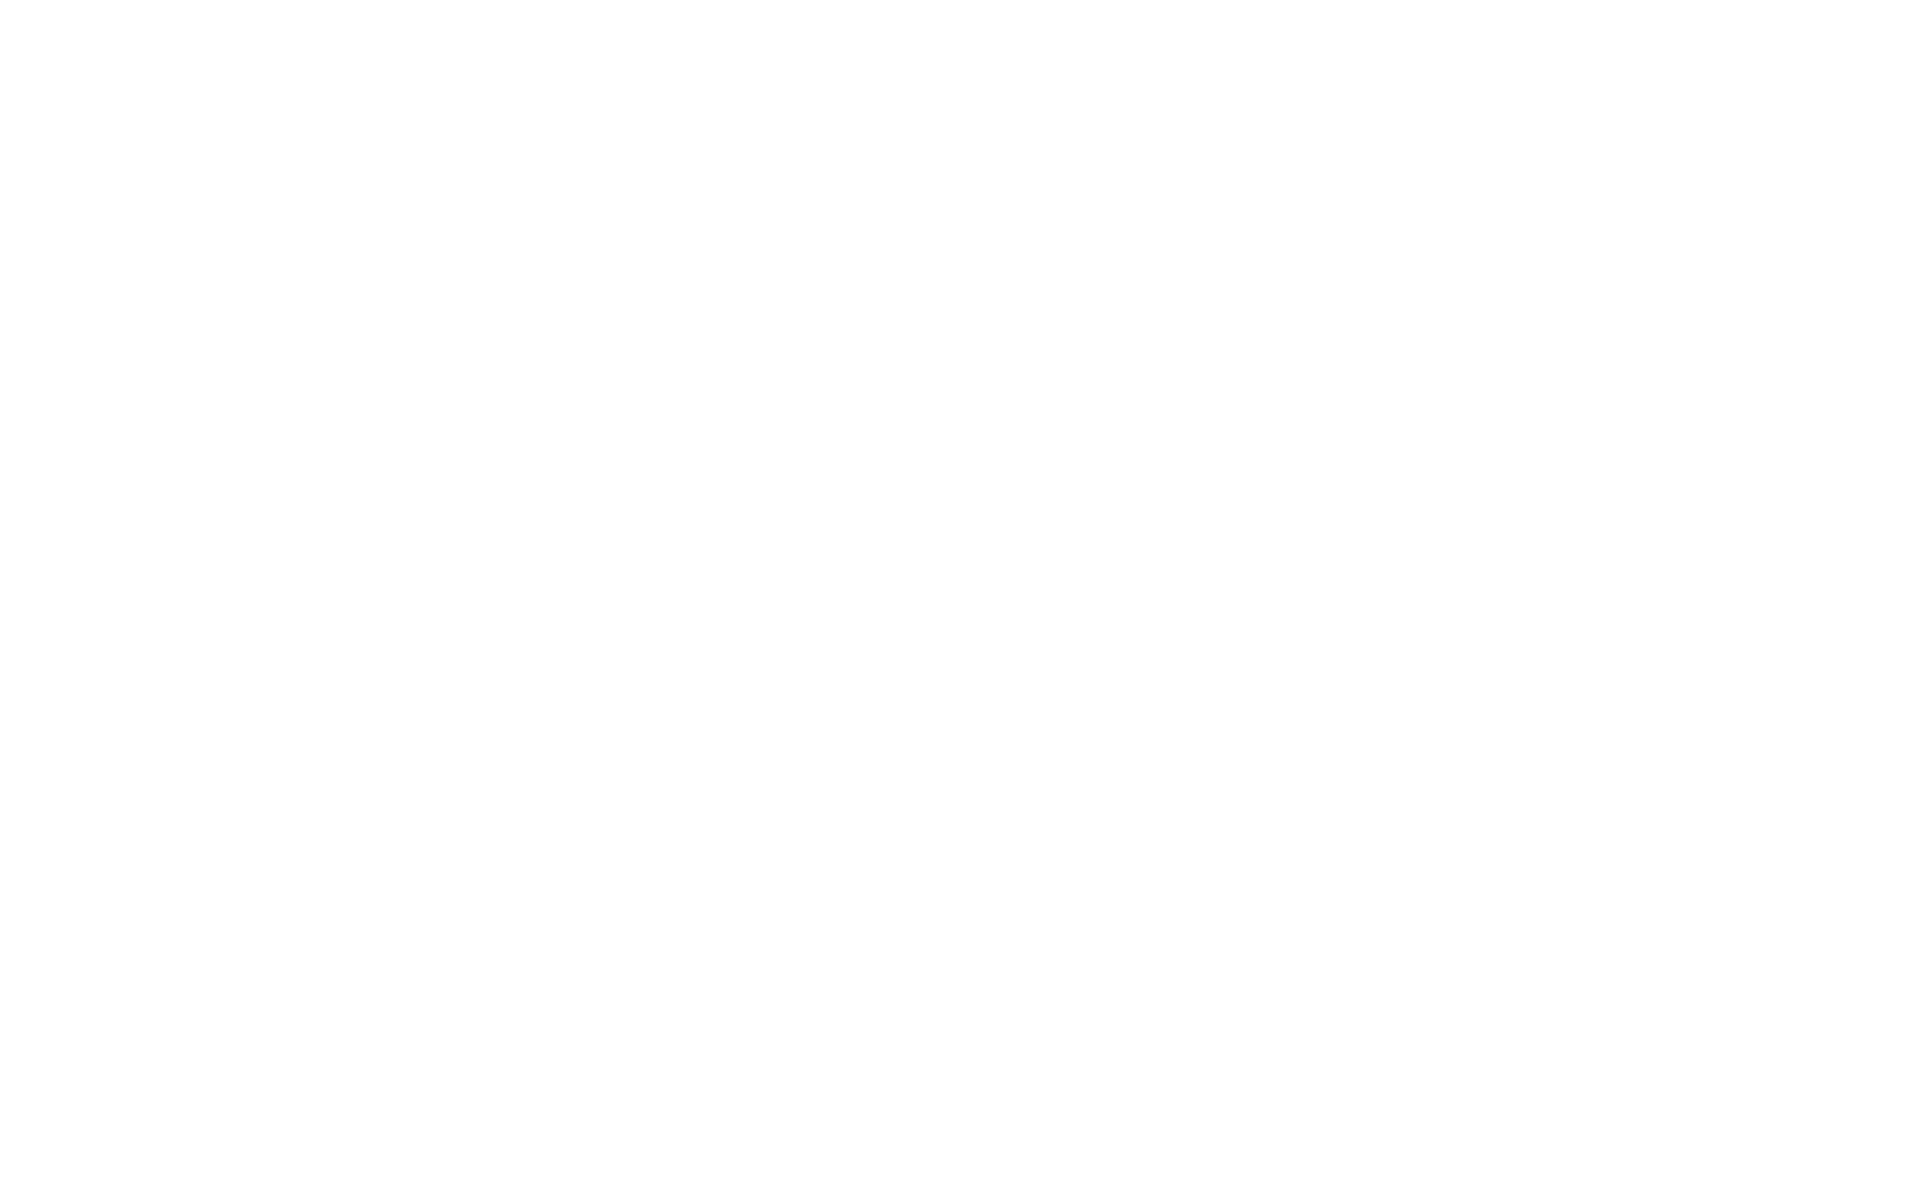
\includegraphics[height=5cm]{img/thank_wikipedia.png}
\end{figure}


\end{frame}

\begin{frame}{NP-hard \emojiflushed}

Intuitively, NP-hard problems are ``at least as hard as the hardest problems in NP''.

\vspace{2mm}

Here are some NP-hard problems:
\begin{itemize}
\item Every NP-complete problem is NP-hard.
\item The \textbf{Travelling Salesman Problem}\footnote{If you haven't heard of it before, search it up! It's useful for food delivery n stuff maybe \emojisushi} is NP-hard; we don't know if it's in NP or not. 
\item \href{https://www.csail.mit.edu/news/super-mario-brothers-isnt-just-hard-its-np-hard}{Super Mario Brothers is NP-Hard}.
\item The Halting Problem 
$$\text{HP} = \{(M, w): \text{$M$ is a TM that halts on $w$}\}$$
is NP-hard, but is known to not be NP, because it isn't even computable!
\end{itemize}

\end{frame}

\begin{frame}{co-NP}

\textbf{Task:} What does ``co'' stand for in ``co-NP''?
\pause
\textbf{Answer:} ``co'' stands for \sout{considering dropping cs} complement.
\vspace{2mm}

\textbf{Definition}: A language $A$ is \textbf{co-NP} if $\overline{A}$ is NP. 
\end{frame}

\begin{frame}{co-NP}
\textbf{Definition}: A language $A$ is \textbf{co-NP} if $\overline{A}$ is NP. 

\vspace{2mm}
Since NP is the set of languages with poly-time verifiers, a language $A$ is in co-NP if and only if there is a poly-time verifier $V$ for its complement:
$$\overline{A} = \{w: \text{there exists $c$ such that $V(w, c)$ accepts}\},$$
or equivalently,
$$A = \{w: \text{there is no $c$ such that $V(w, c)$ accepts}\}.$$

\vspace{2mm}

This means we can \textit{verify that something is not in our language} in polynomial time.
\end{frame}

\begin{frame}{co-NP}

\textbf{Task:} What does ``co'' stand for in ``co-NP''?
\pause
\textbf{Answer:} ``co'' stands for \sout{considering dropping cs} complement.
\vspace{2mm}

\textbf{Definition}: A language $A$ is \textbf{co-NP} if $\overline{A}$ is NP. 
\end{frame}

\begin{frame}{co-NP}
\textbf{Definition}: A language $A$ is \textbf{co-NP} if $\overline{A}$ is NP. 

\vspace{2mm}
Since NP is the set of languages with poly-time verifiers, a language $A$ is in co-NP if and only if there is a poly-time verifier $V$ for its complement:
$$\overline{A} = \{w: \text{there exists $c$ such that $V(w, c)$ accepts}\},$$
or equivalently,
$$A = \{w: \text{there is no $c$ such that $V(w, c)$ accepts}\}.$$

\vspace{2mm}

This means we can \textit{verify that something is not in our language} in polynomial time.
\end{frame}

\begin{frame}{co-NP}
\sout{\textbf{Task:} Answer the following question: is NP = co-NP?}

Actually, we don't know if NP = co-NP. But the following problems are co-NP!
\begin{itemize}
\item pretty much any problem in NP, if you just take its complement. e.g. turn SAT (which asks ``is this formula satisfiable?'') into the problem ``is this formula unsatisfiable?''
\end{itemize}

NOTE: ``co-NP'' is not the same as ``not NP''! Be careful.
\end{frame}


\begin{frame}{yahoot time}
(gotta fill time somehow, there isn't much to cover today though!)

\vspace{2mm}

winner gets (imaginary) \$10 sushi juice coupons. when i open a sushi juice store, you will be able to redeem those coupons.

\begin{figure}[h]
\centering

\includegraphics[width=8cm]{img/helo_fish_kahoot.jpg}
\end{figure}



 
\end{frame}



\end{document}